\documentclass[tikz,border=8pt]{standalone}
\usepackage{amsmath,amssymb}
\usepackage{tikz}
\usetikzlibrary{angles,quotes,calc}

\begin{document}
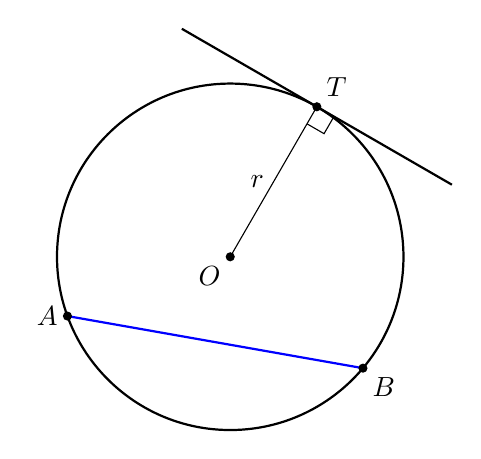
\begin{tikzpicture}[scale=1.1]
  \coordinate (O) at (0,0);
  \def\r{2}
  \draw[thick] (O) circle (\r);
  \fill (O) circle (1.5pt) node[below left] {$O$};

  % Teğet: T noktasında yarıçapa dik
  \coordinate (T) at (60:\r);
  \draw (O) -- node[midway, left] {$r$} (T);
  \coordinate (T1) at ($(T)!1.8cm!90:(O)$);
  \coordinate (T2) at ($(T)!-1.8cm!90:(O)$);
  \draw[thick] (T1) -- (T2);
  \pic[draw, angle radius=2.5mm] {right angle = O--T--T1};
  \fill (T) circle (1.5pt) node[above right] {$T$};

  % Kiriş
  \coordinate (A) at (200:\r);
  \coordinate (B) at (320:\r);
  \draw[thick, blue] (A) -- (B);
  \fill (A) circle (1.5pt) node[left] {$A$};
  \fill (B) circle (1.5pt) node[below right] {$B$};
\end{tikzpicture}
\end{document}
